\chapter{De bewegingssensor  \normalsize{(week 3).}}
\label{chap:bewSen}

De bewegingssensor, welke in rood wordt aangegeven in figuur \ref{fig:motion}, bestaat uit twee hoofdonderdelen, een accelerometer en een kompas. We gaan eerst aan de slag met een voorbeeld dat de bewegingssensor demonstreert, vervolgens met de magnetometer. Waarna beide onderdelen in 1 programma worden bewerkt.
\begin{figure}[h!]
	\captionsetup{justification=centering}
	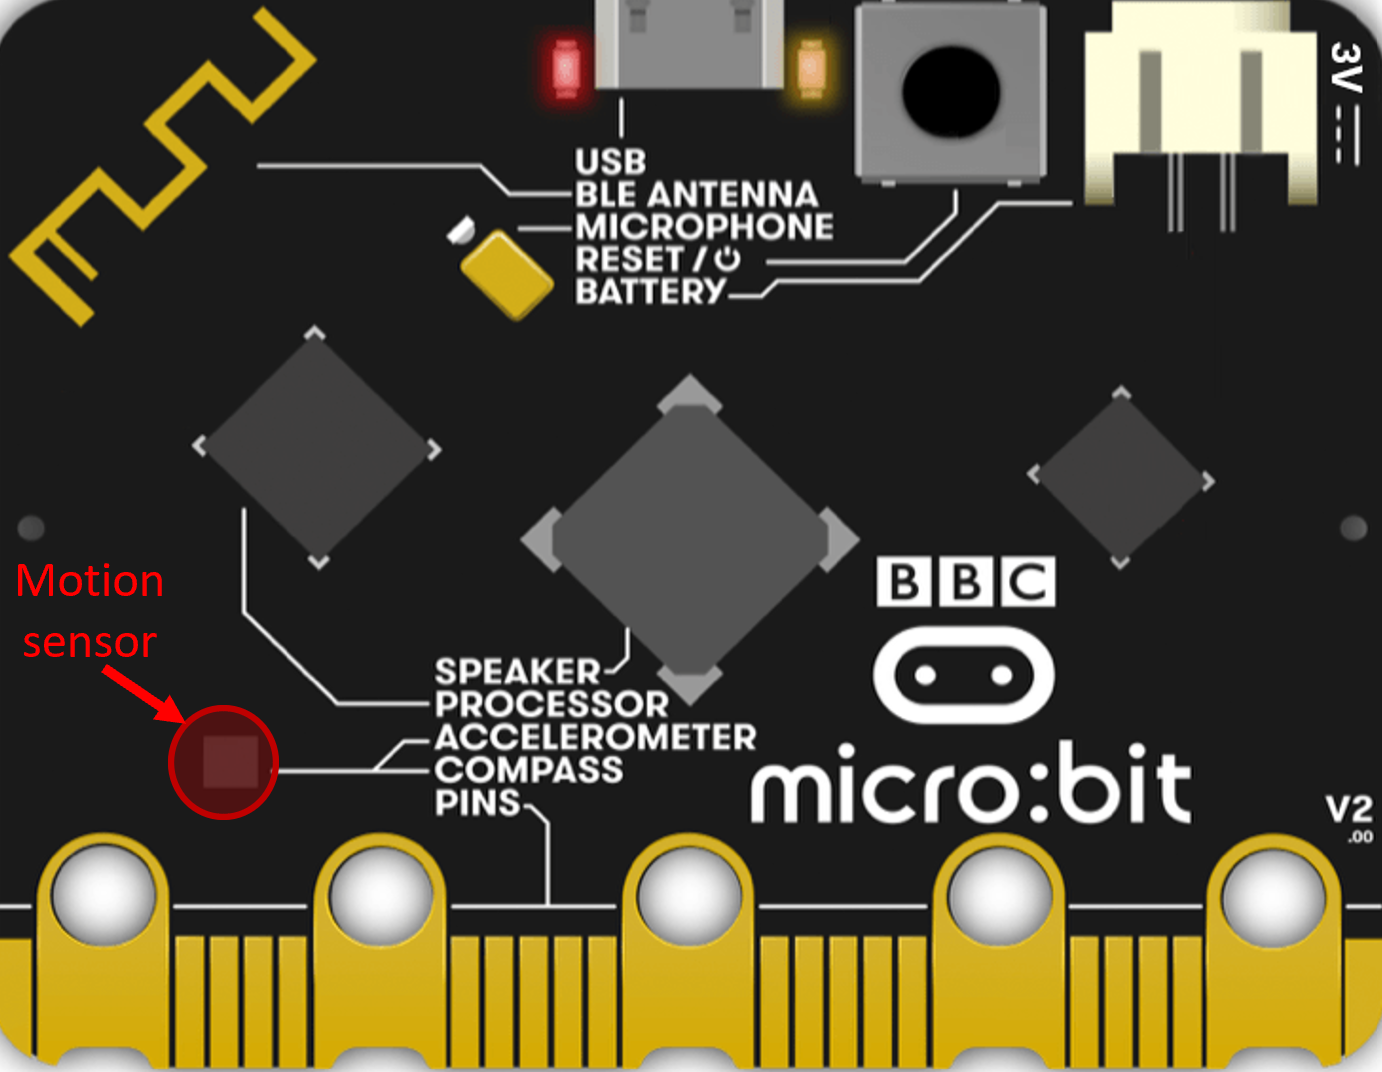
\includegraphics[width=0.2 \linewidth]{figuren/motion}
	\centering
	\caption{Plaats van de bewegingssensor.}
	\label{fig:motion}
\end{figure}

\begin{enumerate}
%	\item  Open Bestand $\rightarrow$ Voorbeelden $\rightarrow$ Microbit-HHS $\rightarrow$ Microbit\_Bewegingssensor\_demo.
\item Installeer de \textit{STM32duino LSM303AGR} library in de arduino. 
Ga naar Sketch $\rightarrow$Include Library $\rightarrow$Manage Libraries of \colorbox{mygray}{\textbf{Ctrl + shift + I}} en type in het zoekveld STM32duino LSM303 zoals te zien is in Figuur \ref{fig:stm32303}.
\begin{figure}[h!]
	\captionsetup{justification=centering}
	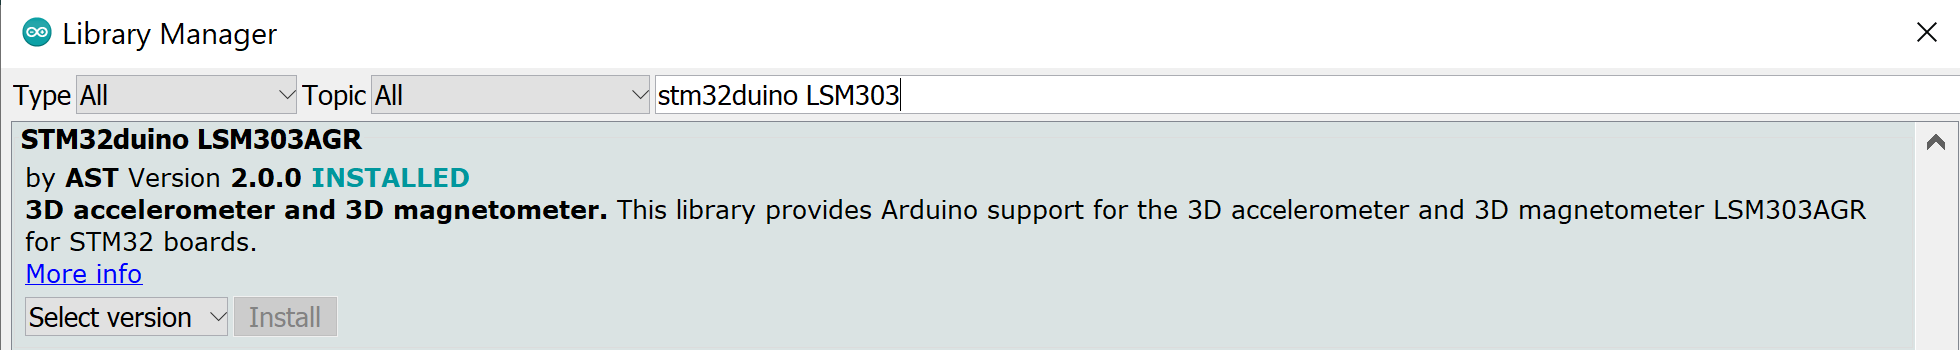
\includegraphics[width=0.6 \linewidth]{figuren/stm32duinoLib}
	\centering
	\caption{Installeren van de STM32duino LSM303AGR.}
	\label{fig:stm32303}
\end{figure}
\item Open het voorbeeldprogramma accelerator.
\item Compileer en upload het voorbeeld naar je Microbit.
\item Als het programma werkt, dan knippert de led linksboven. 
\end{enumerate}

\section{De accelerator}
Stel dat ik in The Challenge de Microbit wil gebruiken om te kijken of de deksel van een container ver genoeg opengaat, dan moet ik dat kunnen meten. De bewegingssensor is daar ideaal voor.
\begin{figure}[h!]
	\captionsetup{justification=centering}
	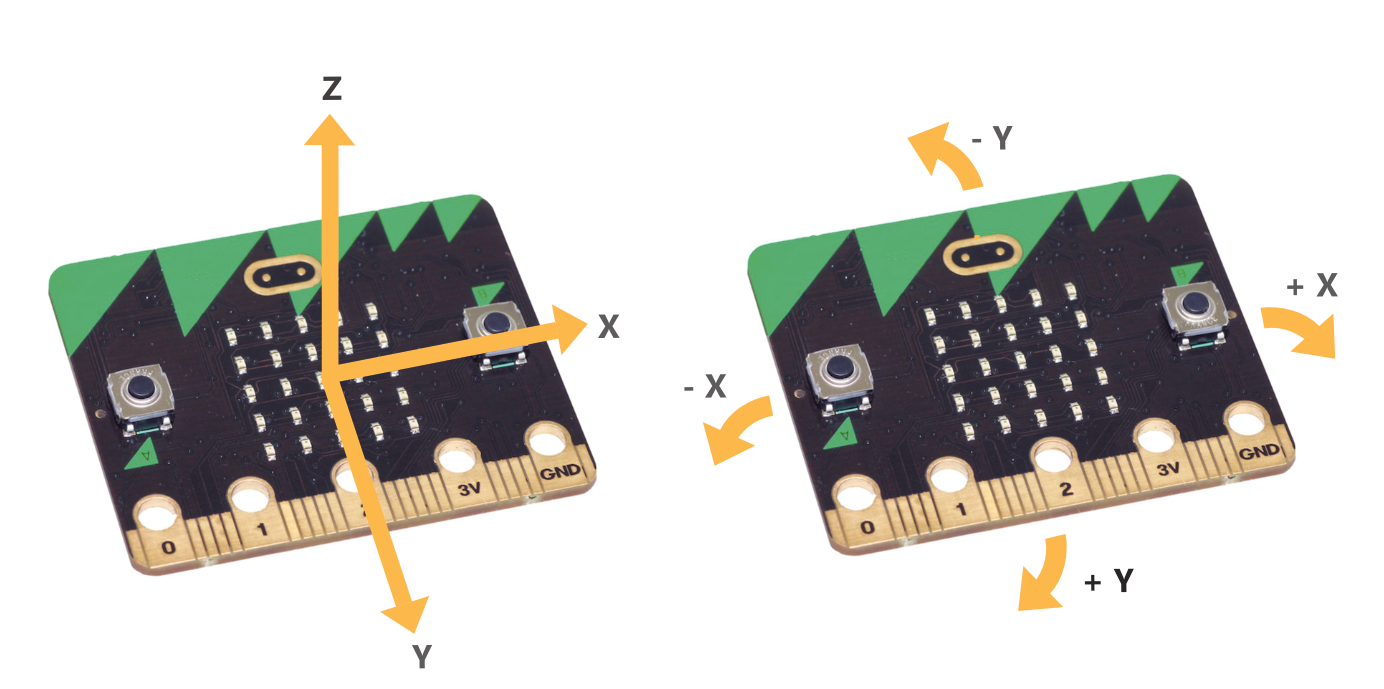
\includegraphics[width=0.35 \linewidth]{figuren/microbit_axes}
	\centering
	\caption{Registratie van de accelerator \cite{microbitAccel}.}
	\label{fig:accel}
\end{figure}
De accelerometer meet de versnelling (beweging) in zowel de X, Y en de Z richting, zoals in figuur \ref{fig:accel} te zien is.

\newpage
De listing van het programma wordt weergegeven in listing \ref{lst:linkaccel}
\begin{lstlisting}[caption={Uitlezen van de accelarator},label={lst:linkaccel}]
#include <LSM303AGR_ACC_Sensor.h>

#define DEV_I2C Wire1   // Wire1 is voor de interne I2C bus 

#define LED ROW1 

// Components.
LSM303AGR_ACC_Sensor Acc(&DEV_I2C);

const int COL1 = 4;   
const int ROW1 = 21;   

void setup() {
	
	pinMode(COL1, OUTPUT);  //aansturing linkerboven LED in matrix
	digitalWrite(COL1, LOW);
	pinMode(ROW1, OUTPUT);
	
	Serial.begin(9600);  	// Initialize serial for output.
	
	DEV_I2C.begin();   	// Initialize I2C bus.
	
	Acc.begin();  	// Initlialize accelarator.
	Acc.Enable();

	uint8_t a;
	Acc.IO_Read(&a,0x0F,1);  //lees waarde Who_am_I register.
	Serial.print("Ik ben: ");
	Serial.println(a);
}

void loop() {
	// Led blinking.
	digitalWrite(LED, HIGH);
	delay(250);
	digitalWrite(LED, LOW);
	delay(250);
	
	int32_t accelerometer[3];
	Acc.GetAxes(accelerometer); 	// Read accelerometer LSM303AGR.
	
	// Output data.
	Serial.print("| Acc[mg]: ");
	Serial.print(accelerometer[0]);
	Serial.print(" ");
	Serial.print(accelerometer[1]);
	Serial.print(" ");
	Serial.print(accelerometer[2]);
	Serial.println(" |");
}
\end{lstlisting}

Op regel 8 wordt een software accelerometer. aangemaakt, die in de \textcolor{OliveGreen}{setup}()  (regel 23 en 24) wordt geïnitialiseerd. In de \textcolor{OliveGreen}{loop}() worden de waarden van de accelerator-sensor opgehaald en in een array gezet (regel 40).  
De opgehaalde waarden worden in de regels 44, 46 en 48 uitgeprint.

Ga als volgt te werk:
\begin{enumerate}
\item Open nu de seriële plotter.
\item Kijk naar de seriële plotter en kantel de Microbit langzaam naar links en naar rechts totdat deze verticaal staat. Doe dat ook naar voor en achter. Draai hem om zijn as. Kijk welke waarde verandert.
\item Zoek een waarde die overeenkomt met de richting die je zoekt, zet de Microbit bijvoorbeeld op zijn rechter zijkant. Je ziet twee meetwaarden die duidelijk meebewegen. Beweeg de Microbit terwijl je hem op zijn zij hebt op en neer. 
%Eén van de twee lijnen geeft een flinke uitslag, de andere niet. Degene die heftig reageren zijn die van de accelerometer, die moet je hebben. Die van de magnetometer reageren ook, maar die zijn afhankelijk van de positie van je Microbit ten opzichte van het noorden (als een kompas). 

\item Bepaal nu (met de seriële monitor) ongeveer de waarde die deze lijn heeft bij een hoek van 45 graden. We maken een aanpassing in het programma zodat deze een melding geeft als de hoek groter is dan 45 graden. In dat geval zetten we de led linksboven aan.
\item \textbf{\underline{Opdracht:}} Zoek de waardes uit en laat de led aangaan boven de 45 graden en weer uitgaan onder de 45 graden. Makkie, toch? Beetje simpel. We gaan meerdere ledjes aansturen.

\item \textbf{\underline{Combineer dit met: Hoe kunnen we de leds (eenvoudig) aansturen?: }}

Open het voorbeeldprogramma \texttt{\textit{heenEnWeer.ino}}. Om dit programma te laten werken zal de 	\href{https://learn.adafruit.com/use-micro-bit-with-arduino/adafruit-libraries}{de Adafruit Libraries}
geïnstalleerd moeten worden. In hoofdstuk \ref{chap:biw} word hier dieper op ingegaan.
%Open Bestand $\rightarrow$ Voorbeelden $\rightarrow$ Microbit-HHS $\rightarrow$ 3B.ForLoopIteration-met-library
\item Compileer en upload het voorbeeld naar je Microbit.
\item Kijk hoe de aansturing van de LEDs werkt en kopieer de benodigde code uit het voorbeeldprogramma \texttt{\textit{heenEnWeer.ino}} naar de bewegingssensor demo. Zorg eerst dat één ledje gaat branden aan de kant waar je de Microbit naartoe kantelt (alsof je een knikker op een dienblad hebt). Breid dit dan uit naar 4 leds (voor, achter, links, rechts) en uiteindelijk naar 8 leds (de leds op de hoeken erbij). 

Als je dit op een echt slimme manier wilt doen, dan gebruik je geen ‘if’ statements maar bereken je de pixellocatie uit de accelerometer waarden. Gebruik dan wel ‘if’ om te clippen.\\
\textbf{Upload het programma op blackboard.}


\end{enumerate}

\section{Het kompas}

Voor het kompas, geldt in principe hetzelfde alleen moet er nu een software-magnetometer aangeroepen worden. Dit kan gedaan worden met het volgende statement:\\
\texttt{\textit{LSM303AGR\_MAG\_Sensor Mag(\&DEV\_I2C);}}\\
Vergeet niet de magnetosensor te includen.\\
\texttt{\textit{\#include \textless LSM303AGR\_MAG\_Sensor.h \textgreater}}

\paragraph{Opdracht:}
Pas Listing \ref{lst:linkaccel} zodanig aan, zodat behalve de accelerator ook de magnetometer wordt aangeroepen en de waarden worden uitgeprint op de monitor. 
\textbf{Upload het programma op blackboard.}

